% %%%%%%%%%%%%%%%%%%%%%%%%%%%%%%%%%%%%%%%%%%%%%%%%%%%%%%%%%%%%%%%%%%%%%%%%%%%%%%%
\documentclass[journal,letterpaper]{IEEEtran}
% include the list of acronyms, math commands and new commands used in this paper
% \usepackage[backend=bibtex,maxnames=2]{biblatex}
\usepackage[pdftex]{graphicx}
%\usepackage[numbers]{natbib}
\bibliographystyle{IEEEtran}
\usepackage{booktabs}
\usepackage{moreverb}
%\usepackage{titlesec}
%\usepackage[titletoc,toc,title]{appendix}
\usepackage{url}
\usepackage{amsmath}
\usepackage{multicol,lipsum}
\usepackage{mathtools}
\usepackage{cuted}
\usepackage{amsfonts}
\usepackage{multirow}
\usepackage{bm}
\usepackage{subfig}
\usepackage{color, colortbl}
\usepackage[colorlinks,bookmarksopen,bookmarksnumbered,citecolor=red,urlcolor=red]{hyperref}

%\usepackage{enumitem}

\hypersetup
{
	pdftitle = {Whole-body control for quadrupedal locomotion on challenging terrain},
	pdfauthor = {Francesco Roscia},
	pdfsubject = {RA-L manuscript},
	pdfkeywords = {legged robots, aerial locomotion, and safe landing},
	pdftoolbar = true,
	colorlinks = true,
	linkcolor = black,
	citecolor = black,
	urlcolor = black,
}

\usepackage[usenames,dvipsnames]{xcolor}%\usepackage{xcolor,colortbl}
\definecolor{blue_iit}{RGB}{51,51,255}
\usepackage{algpseudocode}
\usepackage{algorithm}


\usepackage[acronym,hyperfirst=false]{glossaries}

\usepackage[tight]{units}
\usepackage[normalem]{ulem} % to strike out text, use: \sout{text}
\usepackage{cancel}
\definecolor{Gray}{gray}{0.9}
\usepackage{tensor} 
\usepackage{nicefrac}
%\usepackage{cleveref}
%\crefname{figure}{Fig.}{Fig.}
%\crefname{equation}{Eq.}{Eq.}
%\AtBeginDocument{%
%  \renewcommand{\crefpairconjunction}{,}%% instead of " and\nobreakspace"
%  \renewcommand{\crefmiddleconjunction}{,}% instead of ", "
%  \renewcommand{\creflastconjunction}{,}% instead of " and\nobreakspace"
%}
\usepackage[sorting=none, style=ieee]{biblatex}
\addbibresource{references/bibliography.bib} 
\newacronym{hyq}{HyQ}{Hydraulically actuated Quadruped}

\newacronym{lf}{LF}{Left-Front}
\newacronym{rf}{RF}{Right-Front}
\newacronym{lh}{LH}{Left-Hind}
\newacronym{rh}{RH}{Right-Hind}

\newacronym{haa}{HAA}{Hip Adduction-Abduction}
\newacronym{hfe}{HFE}{Hip Flexion-Extension}
\newacronym{kfe}{KFE}{Knee Flexion-Extension}

\newacronym{imu}{IMU}{Inertial Measurement Unit}
\newacronym{dofs}{DoFs}{Degrees of Freedom}
\newacronym{rt}{RT}{Real Time}

\newacronym{com}{CoM}{Center of Mass}
\newacronym{cop}{CoP}{Center of Pressure}
\newacronym{zmp}{ZMP}{Zero Moment Point}
\newacronym{icp}{ICP}{Instantaneous Capture Point}
\newacronym{cp}{CP}{Capture Point}
\newacronym{cmp}{CMP}{Centroidal Moment Pivot}
\newacronym{grfs}{GRFs}{Ground Reaction Forces}

\newacronym{ls}{LS}{Least Square}

\newacronym{slip}{SLIP}{Spring Loaded Inverted Pendulum}
\newacronym{eom}{EoM}{Equation of Motions}
\newacronym{qp}{QP}{Quadratic Program}
\newacronym{sqp}{SQP}{Sequential Quadratic Programming}
\newacronym{mic}{MIC}{Mixed-Integer Convex}
\newacronym{cmaes}{CMA-ES}{Covariance Matrix Adaptation Evolution Strategy}
\newacronym{ara}{ARA*}{Anytime Repairing A*}
\newacronym{pca}{PCA}{Principal Component Analysis}
\newacronym{cpg}{CPG}{Central Pattern Generator}
\newacronym{wbc}{WBC}{Whole-Body Control}

\newacronym{mpc}{MPC}{Model Predictive Control}
\newacronym{ik}{IK}{Inverse Kinematic}
\newacronym{ocp}{OCP}{Optimal Control Problem}
\newacronym{nlp}{NLP}{Nonlinear Programming}
\newacronym{ltv}{LTV}{Linear Time Varying}


% SOFT TERRAIN ADAPTATION
\newacronym{awbc}{c$^3$WBC}{Compliant Contact Consistent Whole-Body Control}
\newacronym{swbc}{sWBC}{Standard Whole-Body Control}
\newacronym{c3wbc}{c$^3$WBC}{Compliant Contact Consistent Whole-Body Control}
\newacronym{ste}{TCE}{Terrain Compliance Estimator}
\newacronym{c3}{\texttt{c}$^3$}{compliant contact consistent}

\newacronym{stance}{STANCE}{\textbf{S}oft \textbf{T}errain \textbf{A}daptation a\textbf{n}d \textbf{C}ompliance \textbf{E}stimation}

\newacronym{wbopt}{WBOpt}{Whole Body Optimization}


\newacronym{hc}{HC}{Hunt and Crossley's}
\newacronym{kv}{KV}{Kelvin-Voigt's}

\newacronym{wllsr}{WLLSR}{Weighted Linear Least Squared Regression}

\newcommand{\grfs}{\gls{grfs}~}

\newacronym{mae}{MAE}{Mean Absolute Tracking Error}

\newacronym{ode}{ODE}{Open Dynamics Engine}

\newacronym{cmg}{CMG}{Control Moment Gyroscope}
\newacronym{ocs}{OCS}{Orientation Control System}
\newcommand{\reducespace}{\vspace{-1.5em}}
%\newcommand{\reducespace}{\vspace{0em}}
\newcommand{\Rnum}{\mathbb{R}} % Symbol fo the real numbers set
\newcommand{\hf}{\textsc{hf}}
\newcommand{\vect}[1]{\mathbf{#1}} %vector bold

\newcommand{\grf}{F_{\mathrm{grf}}} % vector to denote the contact forces, ground reaction forces
\newcommand{\grfp}[1]{F_{\mathrm{grf,#1}}} % vector to denote the contact forces, ground reaction forces
\newcommand{\grfest}[1]{F_{\mathrm{grf},#1}} % vector to denote the contact forces, ground reaction forces

\newcommand{\mrm}[1]{\mathrm{#1}}
\newcommand{\nmrm}[1]{{#1}}
\newcommand{\fratop}[2]{\genfrac{}{}{0pt}{}{#1}{#2}}
\newcommand{\mx}[1]{\mathbf{\bm{#1}}} 				% Matrix symbol
%\newcommand{\vc}[1]{\mathbf{\bm{#1}}} 					% Vector symbol
\newcommand{\vc}[1]{#1}
\newcommand{\degree}{\ensuremath{^\circ}}				% define the degree symbol
\newcommand{\pder}[2]{\frac{\partial#1}{\partial#2}}		% partial derivative
\newcommand{\refframe}[1]{\mbox{\textless#1\textgreater}}	% to denote a reference frame
\DeclareMathOperator*{\argmin}{\arg\!\min}				% argmin
\DeclareMathOperator*{\argmax}{\arg\!\max}				% argmax
\DeclareMathOperator*{\st}{s.t.}						% subject to
\DeclareMathOperator*{\dif}{\mathrm{d}}					% d
\DeclareMathOperator*{\half}{\frac{1}{2}}					% one half
\newcommand{\mat}[1]{\ensuremath{\begin{bmatrix}#1\end{bmatrix}}}	% matrix
\newcommand{\rank}[1]{\text{rank}(#1)}							% rank
\newcommand{\diag}[1]{\text{diag}(#1)}							% diag
\newcommand{\x}{\ensuremath{\times}}
\newcommand{\dx}[1]{\ensuremath{\delta x_{#1}}}					% dx
\newcommand{\du}[1]{\ensuremath{\delta u_{#1}}}					% du
\newcommand{\DX}[0]{\ensuremath{\Delta X}}						% DX
\newcommand{\DU}[0]{\ensuremath{\Delta U}}						% DU
\newcommand{\ith}[0]{\ensuremath{i^\text{th}}}					% i-th
\newcommand{\T}[0]{\ensuremath{\top}}							% transpose symbol
%\newcommand{\Rv}[1]{\ensuremath{\mathbb{R}^{#1}}}				% set of real-valued vectors
%\newcommand{\R}[2]{\ensuremath{\mathbb{R}^{#1\times #2}}}		% set of real-valued matrices
\newcommand{\Spd}[1]{\ensuremath{\mathbb{S}_+^{#1}}}			% set of symmetric positive-definite matrices
\newcommand*\rfrac[2]{{}^{#1}\!/_{#2}}%running fraction with slash - requires
% math mode.

\newcommand{\crossmx}[1]{\mat{#1}_{\times}} %vector bold

\newcommand\bovermat[2]{\makebox[0pt][l]{$\smash{\overbrace{\phantom{%
    \begin{matrix}#2\end{matrix}}}^{\text{#1}}}$}#2}

\newcommand{\annotation}[1]{\footnote{\color{red}{#1} }}
\usepackage{mathtools}
\DeclarePairedDelimiter{\abs}{\lvert}{\rvert}
\DeclarePairedDelimiterX{\norm}[1]{\lVert}{\rVert}{#1}
\newcommand{\sref}[1]{Section~\ref{#1}}
%\newcommand{\eref}[1]{Eq.~(\ref{#1})}
\newcommand{\eref}[1]{(\ref{#1})}
\newcommand{\fref}[1]{Fig.~\ref{#1}}
\newcommand{\tref}[1]{Table~\ref{#1}}



%\newtheorem{Assumption}{Assumption}[section]
\newtheorem{assump}{Assumption}
\newtheorem{assumpB}{Assumption}
\renewcommand\theassump{1}
\renewcommand\theassumpB{2}
\newcommand{\assref}[1]{Assumption~\ref{#1}}


\newcommand{\MF}[1]{\textcolor{red}{\textbf{mfocchi}: #1}}
\newcommand{\CS}[1]{\textcolor{violet}{\textbf{csemini}: #1}}
\newcommand{\FR}[1]{\textcolor{teal}{\textbf{froscia}: #1}}



\newcommand\BibTeX{{\rmfamily B\kern-.05em \textsc{i\kern-.025em b}\kern-.08em
T\kern-.1667em\lower.7ex\hbox{E}\kern-.125emX}}


\newcommand{\ie}{{i.e.},\ }
\newcommand{\eg}{{e.g.},\ }
\newcommand{\etal}{{\textit{et~al.}}\ }


\captionsetup[table]{labelsep=newline}
\captionsetup[table]{justification=centering}



\makeatletter
\newcounter{definition*}
\newenvironment{definition*}[1][htb]
{\renewcommand{\ALG@name}{Definition}% Update algorithm name
	\let\c@algocf\c@megaalgorithm% Update algorithm counter
	\begin{algorithm*}[#1]%
	}{\end{algorithm*}}
\makeatother

\makeatletter
\newcounter{definition}
\newenvironment{definition}[1][t]
{\renewcommand{\ALG@name}{Proposition}% Update algorithm name
	\let\c@algocf\c@megaalgorithm% Update algorithm counter
	\begin{algorithm}[#1]%
	}{\end{algorithm}}
\makeatother

\newcommand{\defref}[1]{Proposition~\ref{#1}}


%\usepackage[table]{xcolor}
\definecolor{sfahmi_blue}{RGB}{0.19,0.51,0.74}
%\definecolor{DarkGray}{RGB}{0.25,0.25,0.25}
%\definecolor{Gray}{RGB}{0.5,0.5,0.5}
%\definecolor{Red}{RGB}{1,0,0}
\definecolor{LightBlue}{RGB}{0.4,0.4,1}
\newcommand{\thickhline}{\noalign{\hrule height 0.8pt}}

\newcommand{\bmcolor}[1]{\textcolor{RoyalBlue}{\bm{#1}}}


\hypersetup{draft}
\makeglossaries

\title{Reaction Wheels: Enhancing Aerial Maneuvers for
	Legged Robots (Tentative)}
\author{
	Francesco Roscia$^{1}$, Andrea Cumerlotti$^{1, \, 2}$, Andrea Del Prete$^{2}$, Claudio Semini$^{1}$, and Michele Focchi$^{1, \, 3}$
	\thanks{$^1$ Dynamic Legged Systems (DLS) lab, Istituto Italiano di Tecnologia (IIT), Genoa, Italy.
		$^2$ Industrial Engineering Department (DII), University of Trento, Trento, Italy.
		$^3$ Department of Information Engineering and Computer Science (DISI), University of Trento, Trento, Italy.
}}


\begin{document}
\maketitle
\thispagestyle{empty}
\pagestyle{empty}

\begin{abstract}%150-250 word abstract
Aerial motions represent a challenge for quadrupedal robots. They become inevitable to overpass obstacles that cannot be circumvent with standard locomotion gaits. In these cases, the robot must perform a leap to position itself on the obstruction or even flyover it. In this work we propose an \acrfull{ocs} consisting on a couple of rotating and actuated masses (named flywheels or reaction wheels) for the lightweight open-source robot Solo12. Because of the conservation of angular momentum, their rotation can be adjusted to steer the robot base orientation even when there are no contacts with the ground. The axes of rotation of the flywheels are designed to be incident, allowing us to have a compact orientation control system that is capable of controlling both roll and pitch angles of the platform considering the different moment of inertia in the two directions. We proof the concept with simulation and experiments on the real robot.
\end{abstract}

\begin{IEEEkeywords}
	 
\end{IEEEkeywords}

\section{Introduction}\label{sec:introduction}
Legged locomotion is designed for traversing rough terrain.
Different types of gait, such as trot or crawl, have been developed to move quadrupedal robots. 
Thanks to the progress of the last two decades, robots become lighter and able to generate higher torques and forces at the joints, enabling the possibility of doing highly dynamic maneuvers.
Sometimes it is not possible to get around an obstacle with the gaits mentioned above, and jumps may be required. 

When the robot is in air, the \acrfull{com} moves on the ballistic trajectory, that is completely defined by the lift-off position and velocity. On the other hand, the base orientation can be changed exploiting the conservation of the system angular momentum. This means that it is possible to control the base angular velocity by changing the inertia of the robot, e.g., changing the joints configuration. 

Nevertheless, the majority of quadrupeds are designed to respect the massless leg assumption, resulting in limbs having small influence on the total angular momentum.

\begin{figure}[t!]
	\centering
	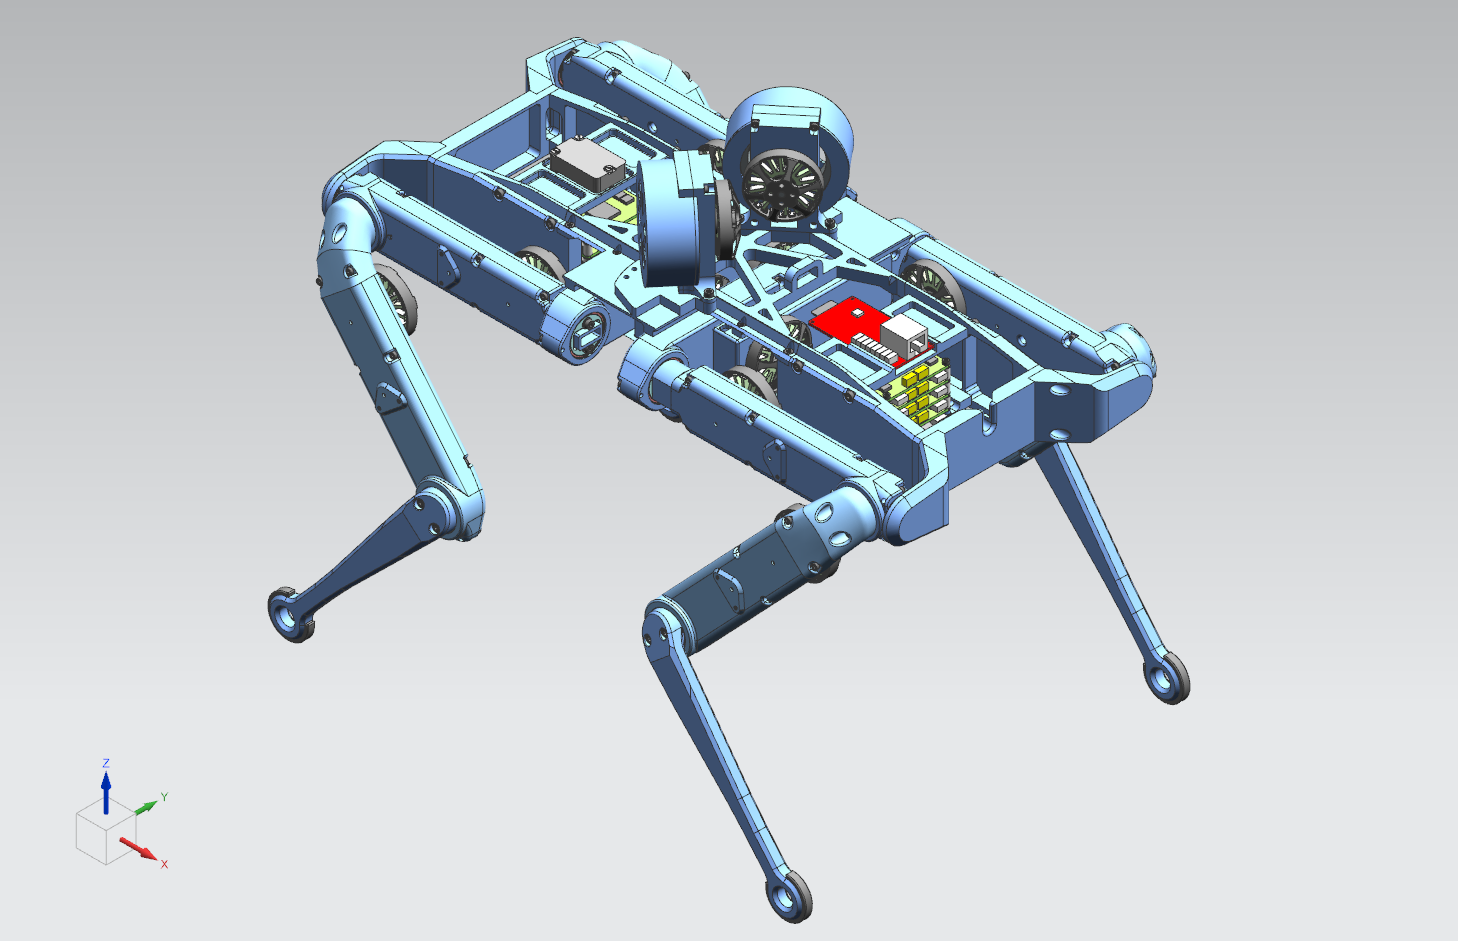
\includegraphics[width=.7\linewidth]{figures/solo_flywheels.png}
	\caption{The \acrfull{ocs} design, having two flywheels with incident rotation axes (magari sostituire con foto)}
	\label{fig:solo12flywheels}
\end{figure} 
\subsection{Related Work}
Quadrupedal animals, like cats, can rearrange the tail and trunk to correct the orientation during a fall \cite{kane1969dynamical}.
% Tail
Many works use an additional link as a tail, like in \cite{chu2019null} and \cite{wenger2016frontal}.
This link rotates around an axis that does not pass through the robot \acrshort{com}: the distances between the axis of rotation and the \acrshort{com} of both trunk and tail allow to obtain large effect on the total angular momentum even with a small tail mass.
However, the placement of the additional link makes the resulting robot asymmetric. Moreover, due to its limited range of motion, a tail can be used only for a single jump, not for a repeated sequence \cite{johnson2012tail}.
% Legs reconfig
It is possible to obtain a similar result by creating repetitive circular motions with the feet, like in \cite{hoffman2021exploiting} and \cite{kurtz2021mini}. In the latter, authors proposes special heavy boots for Mini Cheetah and use a neural network to calculate online joint trajectory. However, this solution unnecessarily increases the inertia of the legs, complicating the locomotion problem.\annotation{trova un modo per dire che questa complicazione è data dalla massless assumption che non è più valida} 
% Gyros
Another option is to use a \acrfull{cmg}.
It consists of a wheel, spinning at a constant angular velocity inside two or three actuated gimbals.
Tilting the wheel's axes of rotation generates the gyroscopic torque.
This system is widespread in spacecrafts reorientation \cite{yoon2002spacecraft}, but less frequently exploited in robot locomotion, either wheeled \cite{brown1996single} or legged \cite{mikhalkov2021gyrubot}.
The \acrshort{cmg} presents interesting capabilities, but the presence of a pan-tilt unit to drive the gyroscope makes impractical to mount it on a small, lightweight robot.

% Reaction wheel
Reaction wheels represent an additional option for controlling the robot orientation.
Changing the angular velocity of a rotating mass attached to the trunk generates a torque that can reorient the robot. Also this device is borrowed by spacecraft orientation \cite{oland2009reaction}, and it was sporadically investigated in legged locomotion for controlling only pitch orientation, both for bipeds \cite{Brown2016}, \cite{xiong2020sequential} and quadrupeds \cite{kolvenbach2019towards}, \cite{vasilopoulos2016quadruped}.
Compared with tails, reaction wheels do not have position limit, and since their rotation axes pass though the \acrshort{com}, its angular momentum results holonomic \cite{machairas2015quadruped}.
To get a fast response, it is necessary to have an abrupt change in the reaction wheel angular velocity (angular acceleration).
Using a brake avoids the employment of a motor able to deliver higher torques \cite{gajamohan2012cubli}, keeping the system compact: the motor slowly accelerates the wheel to a certain speed to store angular momentum and, when a reorientation is required, the break stops its spin.
Since the effect of the break is unidirectional,
a limitation of this approach is given by the fact that it is possible to generate a rotation of the base only in the opposite direction of the reaction wheel angular velocity.

\subsection{Proposed Approach and Contribution}
In this work, we present an \acrfull{ocs} based on two flywheels and mounted on the trunk of the quadruped Solo12 \cite{grimminger2020open}, see Fig. \ref{fig:solo12flywheels}. In order to control roll and pitch orientations with a compact device, the axes of rotation are set to be incident, creating an angle that balances the effect in both the directions. The benefits of the \acrshort{ocs} are the following.
\begin{itemize}
	\item Flywheels can correct orientation errors due to disturbances during the flight and inaccuracies in the angular momentum achieved at the lift-off (e.g., given by tracking issues and non-idealities). 
	\item They enable the robot to land with a desired angular velocity (possibly zero) and orientation.
	In addition, they can enhance the landing phase by significantly reducing oscillations.  
	The presence of these additional joints, whose only function is to control the orientation, gives the possibility to relieve the effort of the legs.
	\item In more complex scenarios, like for a somersault, limbs and \acrshort{ocs} can operate in parallel to achieve a rotation angle larger than the one achievable only with legs (e.g., due to torque limitation). 
\end{itemize}
Furthermore, the \acrshort{ocs} can also be exploited to stabilize dynamic gaits, compensating for trunk oscillations.


\subsection{Outline}
\lipsum[1]
% 

\section{Background}
The starting point for any \acrshort{ocs} is the Euler's equation. For any mechanical system, the time derivative of the angular momentum computed with the respect of with a reference point $O$ fixed in an inertial frame equals
the resultant torque with respect to the same reference point:
\begin{equation}
	\dot{\bm{L}} = \sum_i \bm{M}_i
\end{equation}
When the resultant external moments applied to the system is zero, the Euler’s equation simplifies in
\begin{equation}
\dot{\bm{L}} = 0 \quad \Rightarrow \quad \bm{L}(t) = const.
\label{eq:cons_ang_mom}
\end{equation}
which is known as conservation of angular momentum.
Referring to legged robots, this condition occurs whether the system is not in contact with the ground or other objects, e.g., during a fall or the flight phase of a jump.
In the case, it is possible to change the angular velocity of this base, changing the joints velocities, as a result of the \textit{non-holonomy} of the angular momentum \cite{Wieber16}: if the angular momentum of a certain body changes, the one of the others must modify to maintain the total sum constant.

\section{\acrlong{ocs}}
In the following we present a procedure for selecting the inertia of the flywheels and we show how exploit them to control simultaneously the robot roll and pitch orientation.
\subsection{Inertia Selection}
A preliminary analysis for the selection of the flywheels' inertia can be performed with the Elroy's Beanie model, depicted in Fig. \ref{fig:elroy-beanie}.
\begin{figure}
	\centering
	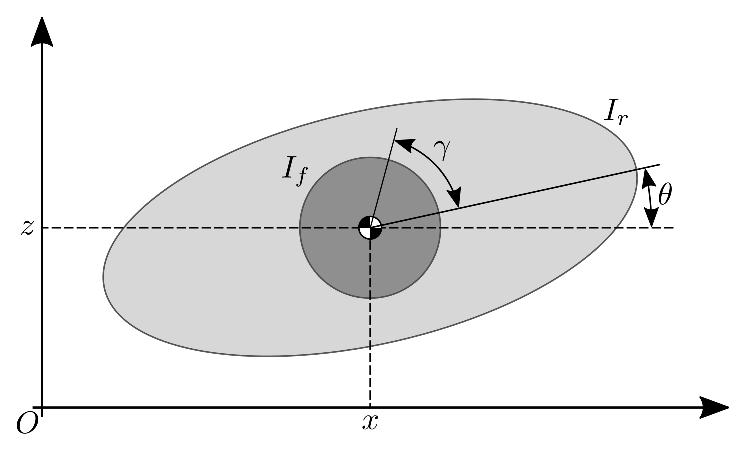
\includegraphics[width=.7\linewidth]{figures/elroys-beanie.eps}
	\caption{Schematic representation of the Elroy's Beanie model used for the preliminary analysis of the pitch motion.}
	\label{fig:elroy-beanie}
\end{figure} 
This consists of two rigid bodies connected through their \acrshort{com} with a revolute joint. One of the bodies represents the robot in its nominal configuration. The other models the \acrshort{ocs}, here represented by a single wheel for the sake of simplicity. The aim is to examine the rotational dynamics of the system as a whole. To simplify the analysis, in the following we will refer only to the effects on the pitch angle of the robot, keeping in mind that the same arguments apply also for the roll. Let identify the moment of inertia of the robot in the nominal configuration as $I_r$ and the moment of inertia of the two flywheels as $I_f$, both referred to system \acrshort{com}.
The angular momentum $L$ of this system can be written as
\begin{equation}\label{eq:ang_mom_elroy}
L(t) = \left(I_r + I_{f}\right)\dot{\theta}(t) + I_{f}\dot{\gamma}(t)
\end{equation}
where $\dot{\theta}$ and $\dot{\gamma}$ are respectively the robot pitch rate and angular speed of the wheel. We want to drive the robot to a desired pitch rate $\dot{\theta}_{des}$ acting on the wheel speed.
Without loss of generalities, we can assume the reaction wheel is stationary with the robot at the instant in which the reorientation maneuver starts ($\gamma_0 = 0$), having a system angular momentum of $L_0 = \left(I_r + I_{f}\right)\dot{\theta}_0$.
Under the condition of conservation of the angular momentum, this quantity is constant over time and it is possible to estimate the lower bound for $I_{f}$ given a desired pitch rate and the maximum velocity of the flywheels $\dot{\gamma}_{max}$:
\begin{equation}
I_{f} \geq \dfrac{\dot{\theta}_0-\dot{\theta}_{des}}{\dot{\theta}_{des}+\dot{\gamma}_{max}-\dot{\theta}_0}.
\end{equation}
Fig. \ref{fig:inertia_limits} reports the lower bound of $I_{f}$ for different initial and desired base angular velocities.
\begin{figure}
	\centering
	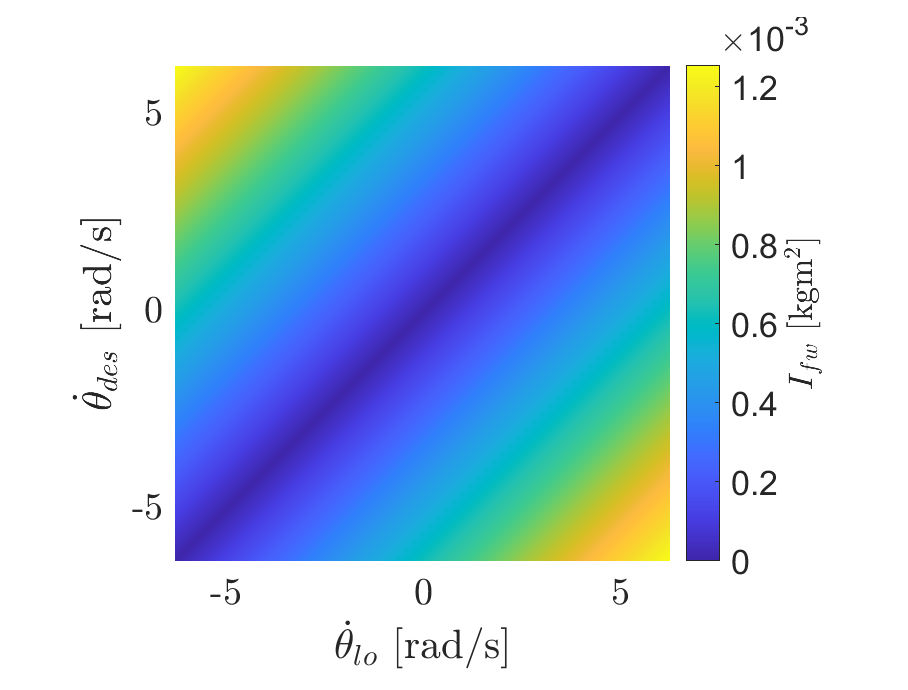
\includegraphics[width=.7\linewidth]{figures/inertia_limits.eps}
	\caption{Minimum inertia necessary to obtain the angular velocity $\dot{\theta}_{des}$ starting with different initial $\dot{\theta}_0$ conditions (questo plot va rifatto)}
	\label{fig:inertia_limits}
\end{figure}

Once the desired inertia $I_f$ is chosen with the 2-D Elroy's Beanie model, it must be used to realize the 3-D object (Fig. \ref{fig:flywheel}). 
\begin{figure}
	\centering
	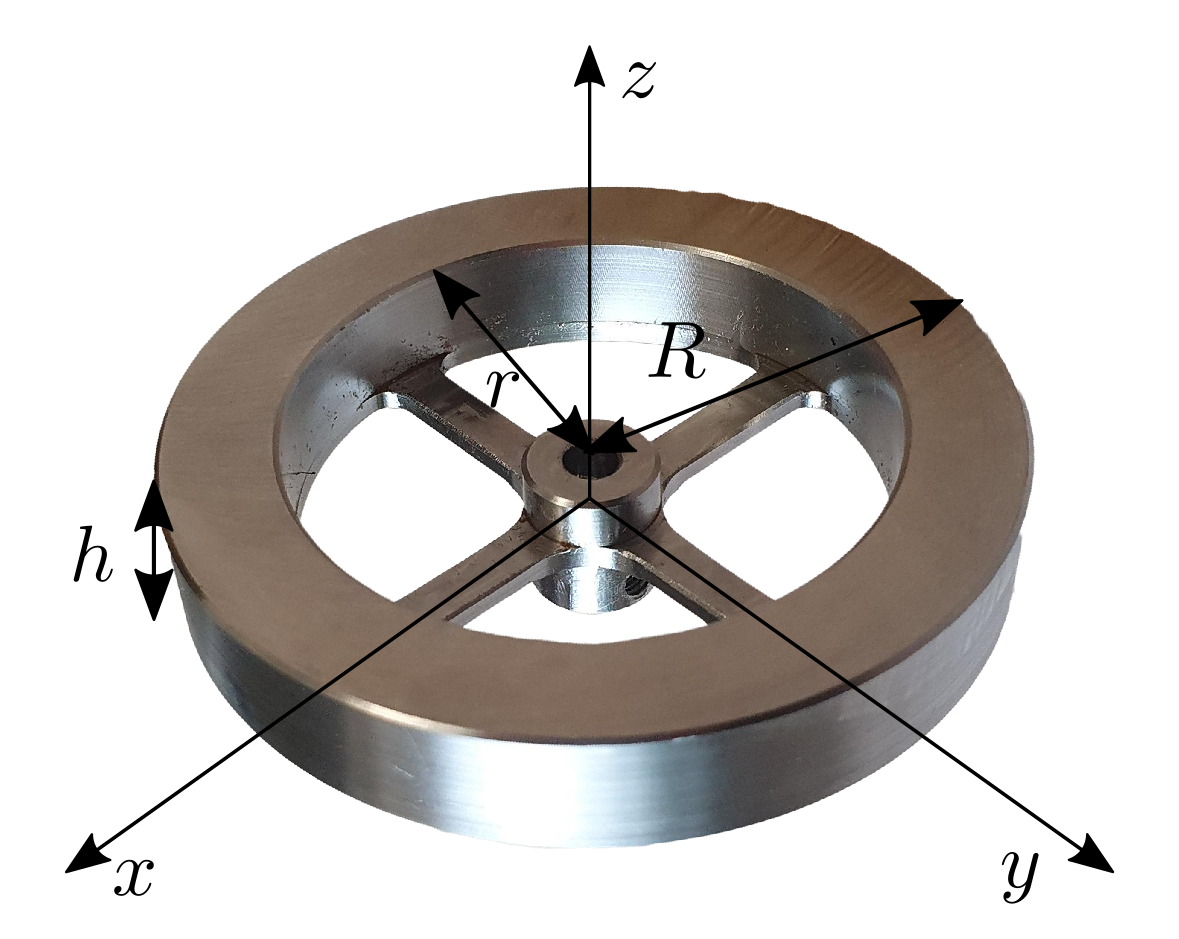
\includegraphics[width=0.7\linewidth]{figures/flywheel.png}
	\caption{The final design of the reaction wheel, shown together with its inertia principal axes. Here, $h$ is the wheel thickness, $r$ is the inner radius of the wheel and $R$ is the outer one}
	\label{fig:flywheel}
\end{figure}
We decided to realize the reaction wheels in the shape of hollow cylinders. This shape increases the inertia locating the mass far away from the rotation axis. The inertia tensor expressed in its principal axes, $\bm{I}_f = \mathrm{diag}\left\{ I_{f, xx}, \, I_{f, yy}, \, I_{f, zz}  \right\}$, depends on the cylinders inner and outer radii, $r$ and $R$, its height $h$ and the material density $\rho$:
\begin{equation}
	\begin{split}
	I_{f, xx} = I_{f, yy} &= \frac{1}{12}\pi \rho h \left(3\left(R^4 - r^4\right) + h^2\left(R^2 - r^2\right)\right) \\
	I_{f, zz} &= \frac{1}{2}\pi \rho h \left(R^4 - r^4\right)
	\end{split}
\end{equation}
Notice that in the Elroy's Beanie model, there is a single body that models the complete \acrshort{ocs}. To met the specification of controlling both the robot roll and pitch, it is possible to select one of two design options:
\begin{enumerate}
	\item use two couples of flywheels, each couple having the rotation axes aligned and orthogonal to the ones of the other couple;
	\item use two flywheels, with incident axes of rotation.
\end{enumerate}
The first case would lead to a bulky \acrshort{ocs}, requiring brakes to achieve relevant angular momentum. Thus, the second option is considered. The inertia introduced in the Elroy's Beanie model have to be split between the two reaction wheels: $I_f = 2 \, I_{f, zz}$.
The parameters $R$ and $h$ can be set to have a compact \acrshort{ocs} and $\rho$ depends on the chosen material, that is stainless steel in our case. The inner radius $r$ can be adjusted to obtain the desired inertia. Spokes with negligible mass connect the wheel to the motor shaft. All the parameters, together with the flywheels final inertia and mass are reported in Table \ref{tab:dim_fw}.
\begin{table}
	\centering
	\begin{tabular}{ccc}
		Parameter & Value & Unit \\
		\hline
		\hline
		$r$ & $2.20\cdot 10^{-2}$ & $\mathrm{m}$ \\
		$R$ & $3.00\cdot 10^{-2}$ & $\mathrm{m}$ \\
		$h$   & $1.02\cdot 10^{-2}$ & $\mathrm{m}$ \\
		$\rho$   & $7.860 \cdot 10^{3}$ & $\mathrm{kg/m^3}$ \\
		$m$   & $1.02\cdot 10^{-1}$ & $\mathrm{kg}$ \\
		$I_{xx}, I_{yy}$   & $3.79 \cdot 10^{-5}$ & $\mathrm{kg \cdot m^2}$ \\
		$I_{zz}$   & $6.92 \cdot 10^{-5}$ & $ \mathrm{kg \cdot m^2}$ \\
	\end{tabular}
	\caption{Size and dynamic parameters of a single reaction wheel}
	\label{tab:dim_fw}
\end{table}

\subsection{Flywheels Axes of Rotation}

The orientation of the axis of rotation of each flywheel influences their contribution to the total angular momentum. To met the specification of controlling both the robot roll and pitch, the axes of rotation of the left and right wheel, identified in the base reference frame with the unit vectors $\hat{\bm{a}}_l$ and $\hat{\bm{a}}_r$, are set to be incident, laying on a plane parallel to the $xy-$ plane of the base reference frame (see Fig. \ref{fig:angVel}). 
To remove unnecessary complications, we design two symmetrical modules. We denote with $\alpha \leq \pi/2$ the non-negative incident angle between the wheels'axes of rotation and the robot lateral direction. The matrix 
\begin{equation}
\bm{C} = 
\left[ \begin{array}{cc}
\hat{\bm{a}}_l & \hat{\bm{a}}_r
\end{array} \right] = 
\left[ \begin{array}{cc}
\sin(\alpha) & \sin(\alpha) \\
-\cos(\alpha) & \cos(\alpha) \\
0 & 0
\end{array} \right]
\end{equation}
maps the reaction wheel moments into scalar torques $\bm{u} = \left[\begin{array}{cc} \tau_{fl} & \tau_{fr} \end{array} \right]^T$ about the flywheel axes $\hat{\bm{a}}_l$ and $\hat{\bm{a}}_r$ (expressed in the base frame).
As long as $\bm{C}$ is full column rank, it is possible to control both roll and pitch angles. If $\alpha = 0$, the roll results to be uncontrollable through the \acrshort{ocs}; otherwise, if $\alpha = \pi/2$, the pitch is not uncontrollable. 
\begin{figure}
	\centering
	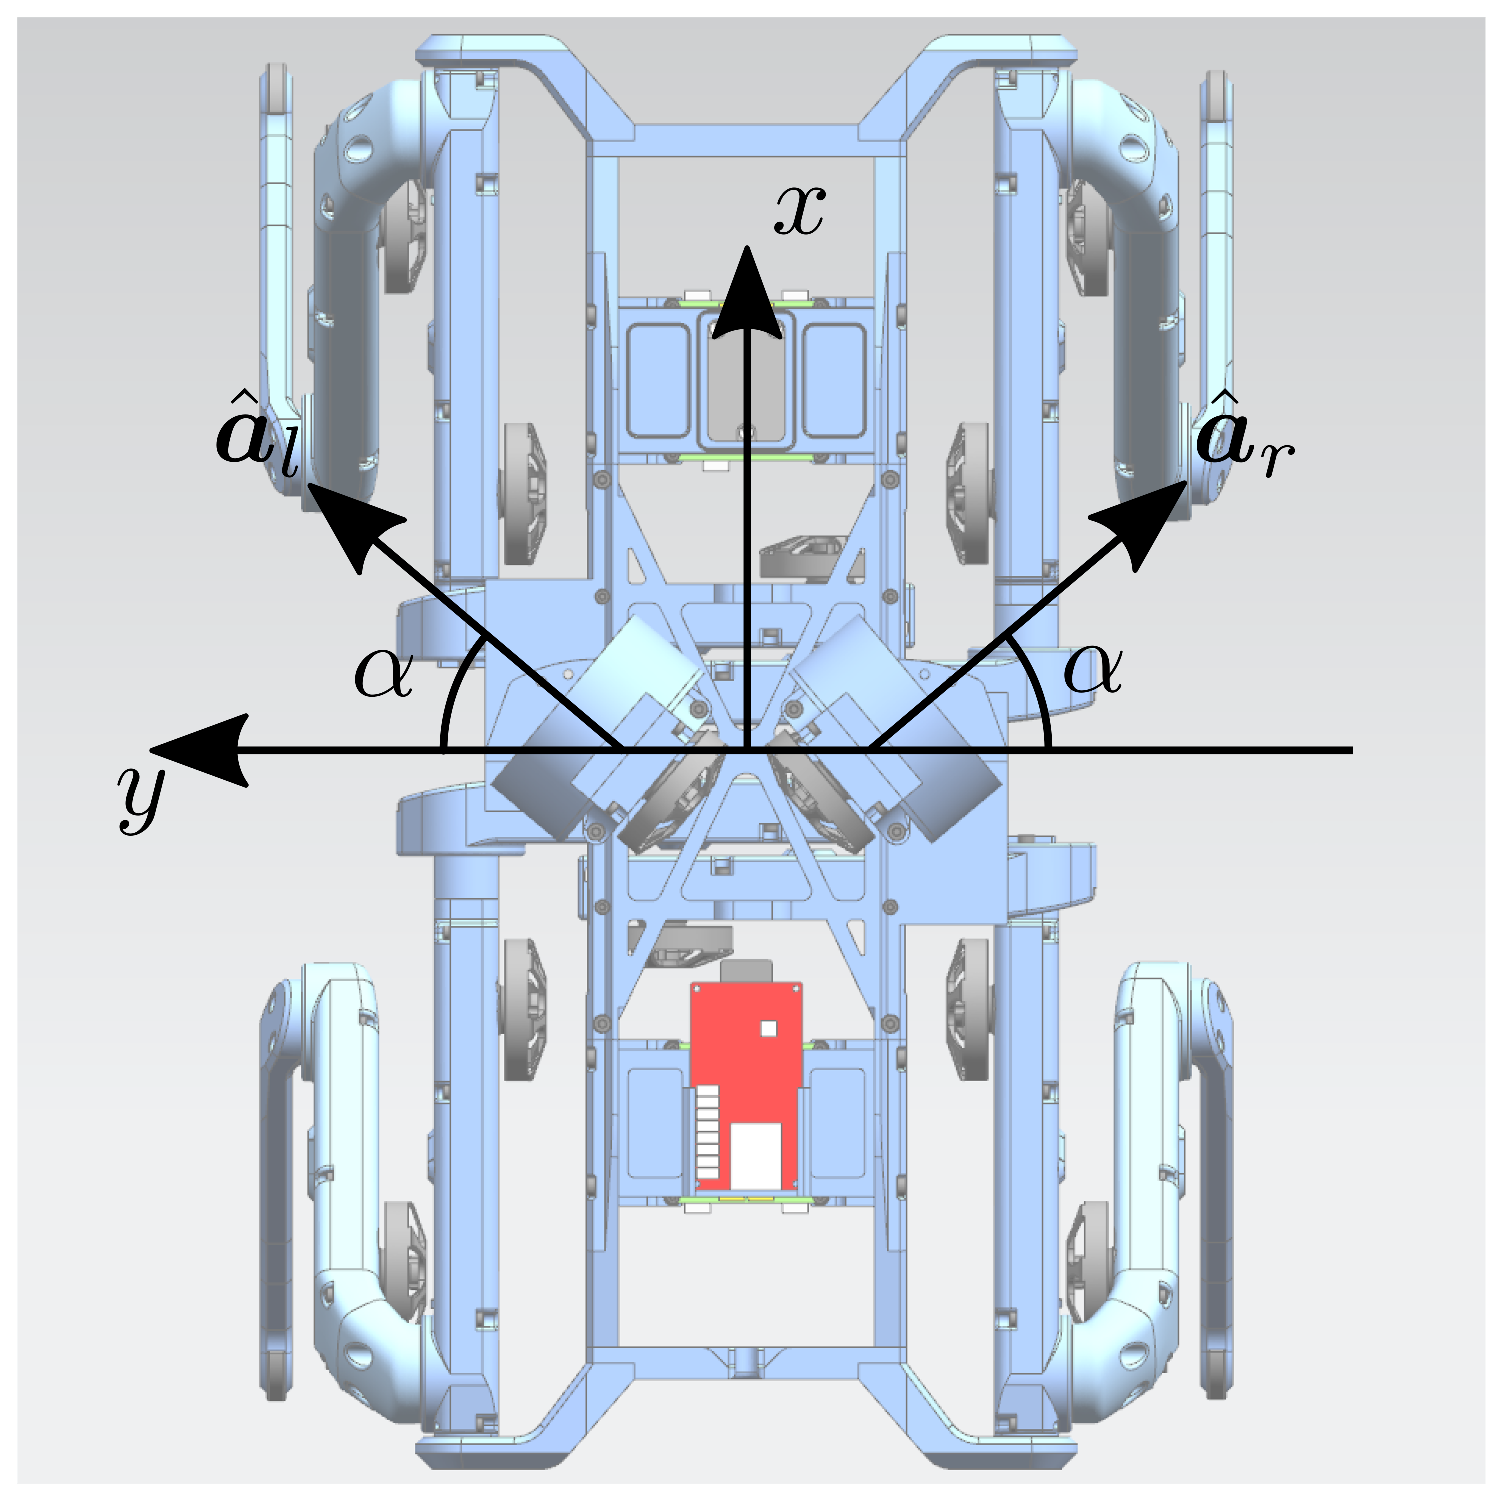
\includegraphics[width=0.7\linewidth]{figures/angular_velocities.eps}
	\caption{Representation of the flywheels rotation axes, seen from the top of the robot}
	\label{fig:angVel}
\end{figure}
The angle is selected considering the ratio of the eigenvalue along the $x$ and $y$ direction of the ellipsoid of the robot inertia:
\begin{equation*}
\alpha^{*}=\tan^{-1}\left(\dfrac{I_{r, xx}}{I_{r, yy}}\right).
\end{equation*}
With these considerations, the angular momentum produced by the left and right wheels expressed in the robot base frame is
\begin{equation}
\begin{split}
\tensor[_b]{\bm{L}}{_f} &= \tensor[_b]{\bm{L}}{_{fl}} + \tensor[_b]{\bm{L}}{_{fr}} \\
&=I_{f, zz} \, \bm{\omega}_{fl} + I_{f, zz} \, \bm{\omega}_{fl}\\
&=I_{f, zz}
\left[\begin{array}{c}
 \left(\omega_{fl} +  \omega_{fr}\right)\sin(\alpha) \\ 
 \left(\omega_{fl} -  \omega_{fr}\right)\cos(\alpha) \\
 0
\end{array}\right]
\end{split}
\end{equation}
in which $\bm{\omega}_{fl}= \omega_{fl} \, \hat{\bm{a}}_{l}$ and $\bm{\omega}_{fr}= \omega_{fr} \, \hat{\bm{a}}_{r}$ are the angular velocity vectors of the two wheels, and $\omega_{fl}$ and $\omega_{fr}$ are the speeds provided to each flywheel by its actuation system. The latter equation shows that the sum of the two angular speed impacts on roll rotations, while their difference can be used to adjust the pitch, see Fig. \ref{fig:sum-dif}. Using the definition of $\bm{C}$, it rewrites as
\begin{equation}
\bm{L}_f = I_{f,zz}
\left[
\begin{array}{cc}
\sin(\alpha) & \sin(\alpha) \\
\cos(\alpha) & -\cos(\alpha) \\
0 & 0
\end{array}
\right]
\left[
\begin{array}{cc}
\omega_{fl} \\
\omega_{fr}
\end{array}
\right] = I_{f,zz} \bm{C} \bm{\omega}_f.
\end{equation}
\begin{figure}
	\centering
	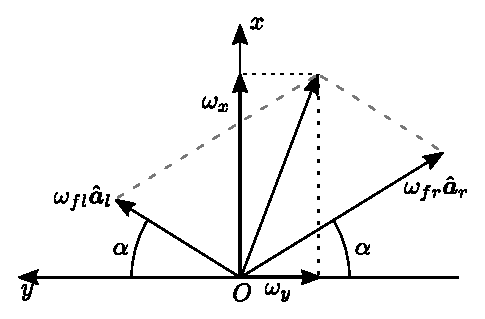
\includegraphics[width=.8\linewidth]{figures/sum_diff.eps}
	\caption{Having incident rotation axes, the \acrshort{ocs} allows to control both the robot roll and pitch. Notice that the roll is influenced by a quantity proportional to the sum of the scalar speed of the flywheels, $\omega_x = \left(\omega_{fl} +  \omega_{fr}\right)\sin(\alpha)$. On the contrary, the pitch depends by a quantity dependent on their difference $\omega_y = \left(\omega_{fl} -  \omega_{fr}\right)\cos(\alpha)$}
	\label{fig:sum-diff}
\end{figure}


\subsection{Flywheels Control Law}
\label{subsec:control_law}
To derive a control law based on the robot base orientation we make use of \eqref{eq:cons_ang_mom}, expressing all the contributions to the time derivative of total angular momentum with respect of the base reference frame:
\begin{equation*}
\bm{I}_f \dot{\bm{\omega}}_f + \bm{I}_b \dot{\bm{\omega}}_b + \bm{\omega}_b \times \left( \bm{I}_b \bm{\omega}_b\right) = 0
\end{equation*}
From this expression we can define the moment on the base caused by the acceleration of the flywheels, that can be used as a feedback torque $\bm{\tau}_{fb}$:
\begin{equation*}
\begin{split}
\bm{\tau}_{fb} &= \bm{I}_f \dot{\bm{\omega}}_f \\
&= - \bm{I}_b \dot{\bm{\omega}}_b - \bm{\omega}_b \times \left( \bm{I}_b \bm{\omega}_b\right)
\end{split}
\end{equation*}
We can use the PD action $\bm{K}_p \bm{e} + \bm{K}_d \dot{\bm{e}}$ to generate a reference acceleration for the base $\dot{\bm{\omega}}_b$.$\bm{K}_p$ and $\bm{K}_d$ are diagonal with positive-definite gains matrices for the error in attitude and angular velocity.
The error $\bm{e} \in SO(3)$ needs the algebra of the special rotational group to be calculated. To avoid singular configurations, we represent the orientation with quaternions.
The derivative error can be calculated using $\dot{\bm{e}} = \bm{\omega}^{des} - \bm{\omega}$, in which $\bm{\omega}^{des}$ and $\bm{\omega}$ are, respectively, the desired and actual angular velocity of the base:
\begin{equation*}
\bm{\tau}_{fb} = - \bm{I}_b \left(\bm{K}_p \bm{e} + \bm{K}_d \dot{\bm{e}}\right) - \bm{\omega}_b \times \left( \bm{I}_b \bm{\omega}_b\right)
\end{equation*}
Projecting $\bm{\tau}_{fb}$ onto the flywheel axes with $\bm{C}^T$ we obtain the control action $\bm{u}$
\begin{equation}
\label{eq:ctrl_law}
\bm{u} = \bm{C}^T \bm{\tau}_{fb}
\end{equation}

\section{Simualtions and Experimental Results}
To validate our \acrshort{ocs}, we present three simulations on different scenarios. We want to test the abilities of: dumping trunk oscillations after the touch down, rejecting disturbance when the robot is in the flight phase of a jump, and working in parallel with the legs joints to achieve an highly dynamic motion. All the simulation are performed in Gazebo. The robot full dynamics is modeled with Pinocchio \cite{carpentier2019pinocchio} the legs joints references are computed off-line using Crocoddyl \cite{mastalli2020crocoddyl} and tracked with a PD joint controller. The \acrshort{ocs} are commanded to track base orientation references using the control law introduced in \ref{subsec:control_law}.

In the first test, we use the \acrshort{ocs} to dump the base oscillations generated at the landing, even though we designed it to control the orientation during the flight phase.
To demonstrate this feature, we use the same joint trajectory to perform two simulations: in the first, we control the reaction wheels to track an orientation parallel to the ground, while in the other they are not actuated.
The joint trajectory realizes a jump with a height of $0.4 \ \mathrm{m}$, a forward distance of $0.8 \ \mathrm{m}$, and a flight phase of $0.5 \ \mathrm{s}$.
The results point out the possibility of using this device even when the angular momentum is not conserved.

The necessity of having an \acrshort{ocs} is faced up in the case of disturbance that occurs when the robot has no contact with the ground. During the flight phase of a forward jump, a purely angular external momentum on the robot base deflects its orientation trajectory: this disturbance is set to $\dot{\bm{L}}_{b, dist} = \left[\begin{array}{ccc}
0.2 & 0.8 & 0.0
\end{array}
\right]^T \ \mathrm{N \cdot m}$ and applies for $0.05 \ \mathrm{s}$. If the flywheels are kept stopped, Solo12 inevitably falls after the touch down. Instead, pairing the legs joint PD controller with \ref{eq:ctrl_law}, it is possible to drive the robot to a safe configuration after the landing.

We carry out a simulation with Moon gravity ($1.62 \ \mathrm{m/s^2}$).
In this way, it is possible to obtain high jumps with a long flight phase.
The leg joint trajectory computed offline describes a vertical jump of $1 \ \mathrm{m}$, having a flight phase that lasts $2 \ \mathrm{s}$.
Right after the lift-off, the reaction wheels start the reorientation task of performing a somersault, i.e., a spin of $360^\circ$ on the pitch.
For this maneuver, the ideal value of the incident angle $\alpha$ is $0^\circ$ since no roll rotation is required, and it is preferred to use all the contributions of the \acrshort{ocs} on the pitch.
Our design allows the manual change of this value before the task starts.
This simulation demonstrates that reaction wheels alleviate the effort to be applied on the legs, which are only used for linear motion.


\section{Conclusions}
\label{sec:conclusion}

\small
\section*{Acknowledgements}	



\printbibliography
\end{document}